HTBAC is a Python-implemented workflow system \jhanote{Do you mean a workflow
management system? Is it really a workflow (management) system? What are the
essential properties of a workflow management system?} that sits between the
user and cyberinfrastructure \jhanote{"sits between user and
cyberinfrastructure" is too colloquial. is it a library? is it a runtime
module?} in order to scale \jhanote{in order to scale: scale what?} and
investigate free energy protocols with a variety of physical systems. HTBAC
allows to encode binding free energy protocols, such as ESMACS and TIES, into
ensemble applications\@. A protocol in HTBAC encoded as an ensemble of
pipelines comprised of identical sequence of stages.
\jhanote{ensemble of replicas is redundant. a replica is an ensemble member,
and an ensemble is by definition comprised of ensemble members. the question
is what is that ensemble member. here it is a pipeline of ... }

\jhanote{the definition of protocol profferred here is too generic: e.g., per
definition of protocol above it is unclear if "interacting" replicas would be
covered?}
\jdnote{As per ESMACS and TIES, the replicas are non-interacting. Ensembles
can be interacting but as per ESMACS/TIES protocols the replicas are not
required to be interacting.} \jhanote{I think this is narrow/constraining: we
have discussed how replica exchange might be a future protocol}

We express the application logic of HTBAC using the user-facing API of EnTK
(\S\ref{ssec:entk}). The EnTK API and its programming model allow HTBAC to
express the workflows associated with different protocols as ensemble-based
applications.

\jhanote{lets get the definition and description clear, then we can come back
and describe the advantages} \st{minimizing development effort and complexity.}


An ensemble of replicas in the ESMACS and TIES protocol directly maps to a set of
pipelines in EnTK, where each replica maps to a single pipeline consisting of
a sequence of stages. Each stage consists of a task
\mtnote{each stage has only one task as specified in the following paragraph}
\jdnote{done} that perform unique functions including preprocessing and
molecular dynamics simulations. 

% directly to a set of pipelines in EnTK, where each pipeline contains
% functions that operate on a given replica. EnTK interprets these replicas
% as independent pipelines. Each pipeline consists of multiple stages
% representing a well-defined execution order; each stage can contain
% heterogeneous workloads. Although each stage of a pipeline depends on its
% predecessor, the pipelines execute independently of each other.
ESMACS and TIES protocols differ in the details of the pipelines, stages and
synchronization~\cite{Bhati2017}. 
% The patterns
% \jhanote{what is a pattern within a pipeline? a pipeline is a pattern by
% some accounts?} within pipelines; however, are identical and describe an
% ensemble of replica simulations.
Fig~\ref{figure:HTBAC} % demonstrates 
shows how pipelines, stages and tasks are organized for the ESMACS
protocol.

% \mtnote{I am afraid we need to iterate the whole pragraph. We need to
% separate between the abstracitons used in the ESMACS protocol (replica,
% function, simulation) to those of EnTK (pipeline, stage and task). Once
% separated, we need to map the former into the latter.} \jdnote{better? also
% see caption of HTBAC figure}

\begin{figure}
\centering
  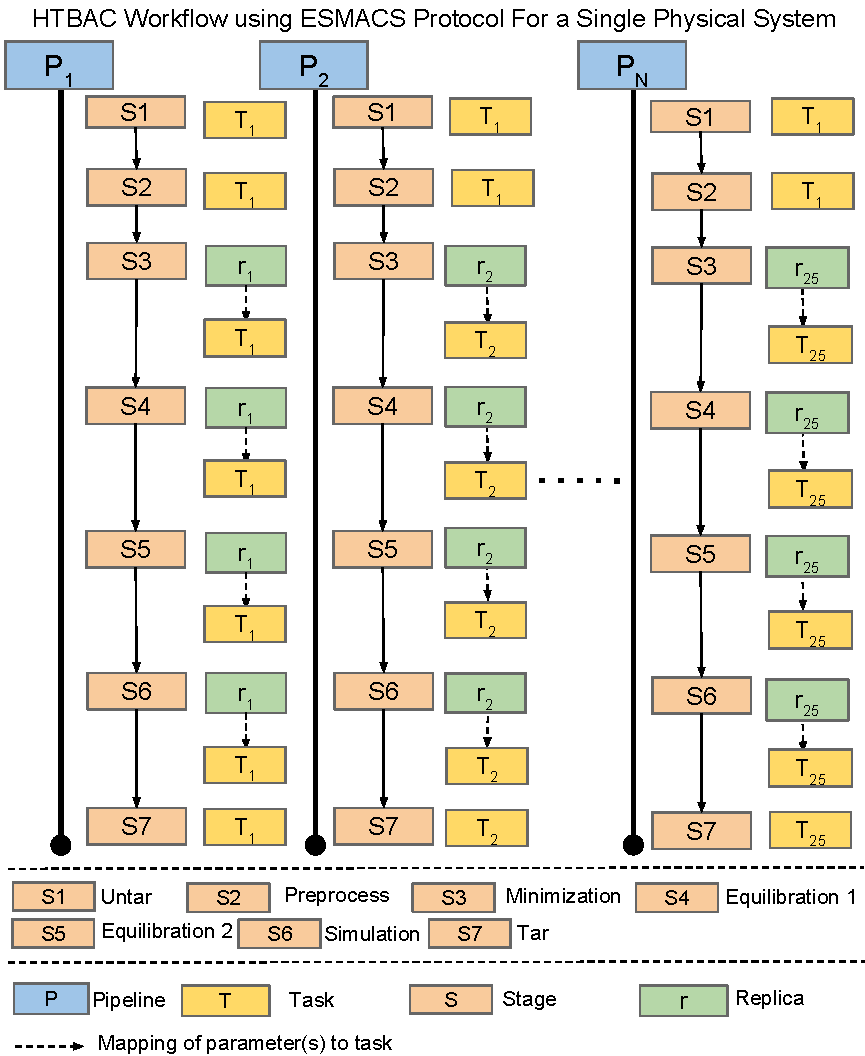
\includegraphics[width=0.5\textwidth]{FIGURES/HTBAC_Workflow_ESMACS.pdf}
  \caption{ESMACS protocol implemented as an HTBAC
  application \mtnote{application?} \jdnote{done}, encoded using the EnTK % PST model
  API \mtnote{If you accept my suggestion to comment out `PST
  model' and instead use API, then that note is not required}. \jdnote{done}. 
  Each protocol represents a physical system and is % captured 
  encoded as a set of independent pipelines. Each pipeline maps to a single
  replica, where ESMACS consists of 25 replicas. Stages within a pipeline
  % maintain temporal ordering
  are executed sequentially. Each stage contain a task \mtnote{each stage has
  only one task as specified in the following paragraph} \jdnote{done} performing unique
  functions, as required by the protocol. Stages S3--S6 contain molecular
  dynamics simulation tasks executed with NAMD\@.}\label{figure:HTBAC}
\end{figure}

% The ESMACS protocol consist of pipelines with stages comprised of
% heterogeneous tasks. For example, equilibration and production, followed by
% post processing steps. 

% \begin{figure}
% \centering
%   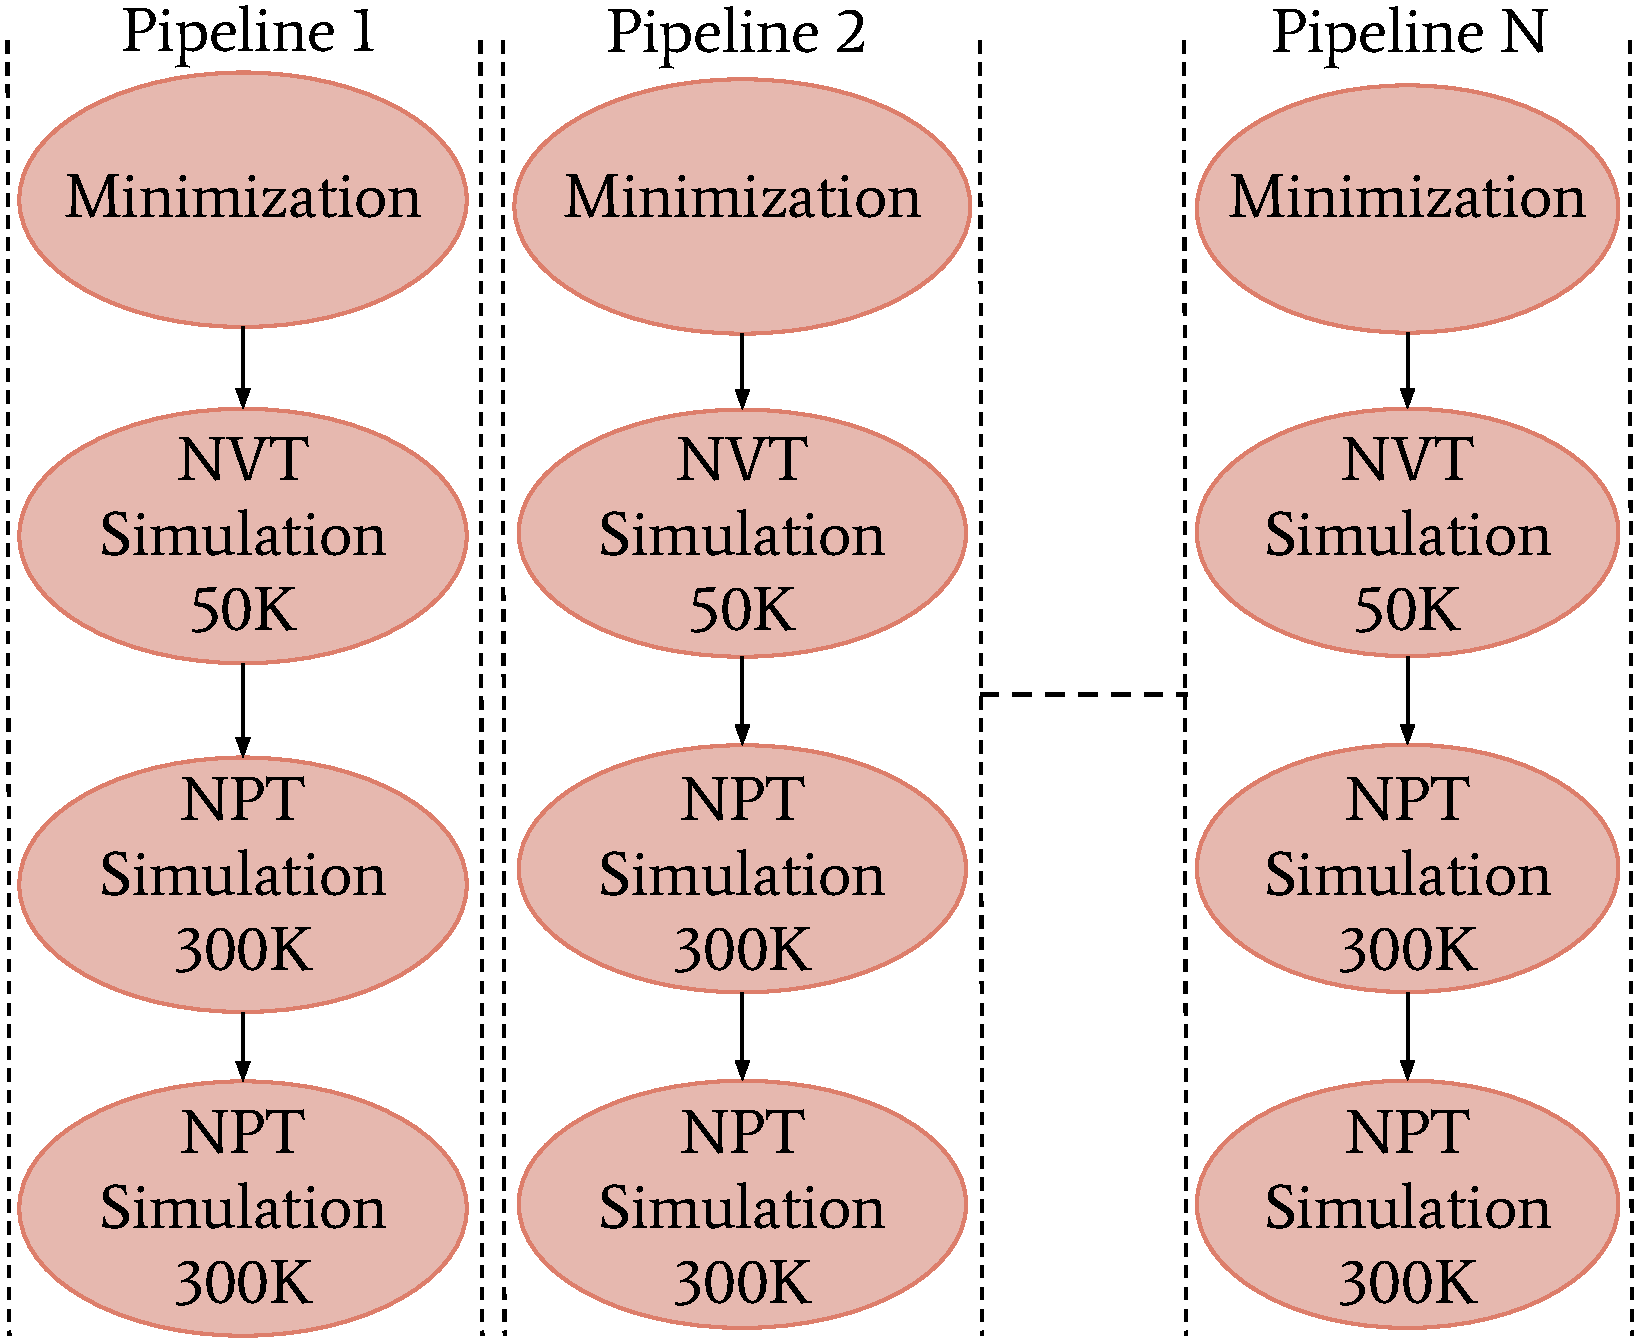
\includegraphics[width=0.5\textwidth]{FIGURES/HT-BAC_NAMD_pipelines_control_flow_only.pdf}
%   \caption{ESMACS protocol indicating how an N replica ensemble is implemented in HTBAC.
%   Each protocol instance is mapped to a single EnTK pipeline.
%   Each pipeline is equivalent and represents a set of simulations which are captured as stages by
%   EnTK.}\label{figure:ESMACS-pipelines}
% \end{figure}

%\begin{itemize}
%	\item 1) Untar configuration files
%	\item 2) Preprep
%	\item 3) Minimize with decreasing restraints
%	\item 4) Equilibration: NVT simulation at 50K, with restraints
%	\item 5) Equilibration: NPT simulation at 300K, with decreasing
%	restraints
%	\item 6) Equlibratin: NPT at 300k, no constraints
%	\item 7) Tarball output files
%\end{itemize}

Each stage is composed of a single % unique 
task with
% which is described by 
a set of attributes that define % the workload 
parameters % such as 
like the location of input files, the number of simulations and the MD
engine(s) used to launch those simulations. The ESMACS protocol % defines 
has 7 stages: %, in which 
the first, second and last stages perform staging of the input/output data,
the middle stages indicate simulation tasks as shown in
Fig~\ref{figure:HTBAC}. The task is appended to a stage and stages are
appended to a pipeline to maintain temporal order during execution. 

% \mtnote{I notice that in the experiment section we write: ``where stages
% 1,2, and 7 perform file movements, while stages 3,4,5, and 6 execute NAMD
% tasks.'' Should we edit the previous sentence accordingly?} \jdnote{fixed}

% \mtnote{The following should be edited for readability and probably
% separated into a new paragraph. Note how we introduce `resource
% configuration' here and we use it again in the following paragraph.}

We capture the integration of the application (ESMACS protocol) and how it
interfaces with EnTK in Fig.~\ref{figure:ht-bac_rp}. HTBAC provides methods
for the user to specify a resource request including walltime, cores, queue,
and user credentials. EnTK converts the HTBAC workflow into a set of tasks
called compute unit descriptions and submits them to RP, along with the
resource request. RP uses SAGA to submit a job to the specified queue in the
batch system of the HPC machine. Once the job is scheduled by the batch
system, the pilot becomes active, and it bootstaps the Agent module of RP\@.
The Agent communicates with the MongoDB database (RP DB), and pulls compute
unit descriptions in bulk. Once resources become available, the compute unit
descriptions are translated into executable units and spawned for execution.
\jhanote{I do not think the last few sentences in the paragraph above are
relevant to HTBAC. A HTBAC user/developer used EnTK and should know nothing
below that. As an HTBAC user I would be justified in not knowing anything about
SAGA and RP!}
\jdnote{We have Fig.~\ref{figure:ht-bac_rp} just below that describes the 
integration of HTBAC, EnTK, RP. We mention the Agent, RP DB, Tasks, CUs, 
Pipelines, etc. Therefore, I included a brief description of these 
components, or else the reader would be left wondering what these components are.}
\jhanote{the reader will still be left wondering what an Agent is, what SAGA
is. These are not described or discussed anywhere in the text!}

\jhanote{At the end of this section the reader still does not know what HTBAC
is? Also, the reader knows what HTBAC enables, but not how.}
\jdnote{Not entirely sure if I understand this comment, I added a line at the 
beginning of this section to see if this is the path you're referring to. Also
added a sentence below to address how}\jhanote{My comment is that we've not
still described whether HTBAC is a set of scripts or a library? client side
software or server side? etc.}

Once the HTBAC workflow is expressed, the user is able to define and assign
a physical system to a specific protocol along with the number of replicas.  
\jhanote{I think the workflow description includes the protocol, the number of
replicas and physical system. These are not defined after the workflow.} 

\jhanote{I would  move this to the opening paragraph of this section: } HTBAC
is designed to provide scalable implementations of protocols to enable
multiple, concurrent binding affinity investigations of different physical
systems and mutations.


% \jdnote{Better?}\mtnote{further iterated.}

% When the job gets scheduled by BW, the job is given resources, and the
% first thing done is to bootstrap the agent. The Agent is bootstrapped and
% the first component (data staging). It calls the RP DB and pulls in bulk
% the avaialble CUs checks the properties of input files. THe units are ready
% for scehdulidng, passes it to the queue of the scheduler, it pushes them to
% the queue of the agent scheduler. The executor manages one unit at a time.
% When there is a unit in the queue (inptu staging) and spawns it to the BW
% executor (APRUN). The executor (agent) waits for a the unit to return,
% passes the unit to the output staging, and informs the scheduler.

% \begin{figure}
% \centering
%   \includegraphics[width=0.5\textwidth]{FIGURES/HT-BAC_NAMD_pipelines_contr
%   ol_flow_only.pdf}
%   \caption{\bf NAMD Stages of HTBAC ESMACS protocol.}
%   \label{figure:ESMACS-pipelines}
% \end{figure}

% We define the client resource in Fig.~\ref{figure:ht-bac_rp} as the workload
% system---HTBAC\mtnote{I do not understand this sentence. Some problems I see
% with it: I do not see a definition if Fig. 4; what is a `client resource'?
% What is a `workload system' in this context?} which describes a set of
% replicas with ordered functions as pipelines with stages and tasks
% \mtnote{The rest of the sentence seems to use functions as previously done in
% the opening paragraphs?}. EnTK interprets these pipelines as a functional set
% of tasks \mtnote{I am not sure I understand what a `functional set of tasks'
% is} and generates the pilot description that contains the resource
% configuration of how to run the HTBAC workload. For the ESMACS protocol
% running on Blue Waters we define the runtime system, queue, and the pilot
% size. Once RADICAL-Pilot receives this new workload, it generates a pilot
% that submits placeholders to the queue \mtnote{A pilot is a resource
% placeholder. The sentence needs editing.}. Once the pilot % is activated
% becomes active, the RP-Agent submits the tasks in the form of compute units
% to the placeholders to begin execution \mtnote{RP-Agent is the pilot and
% therefore the resource placeholder. Let's discuss in person about RP
% execution model and how it is implemented by both RP modules and
% components}.

\begin{figure}
\centering
  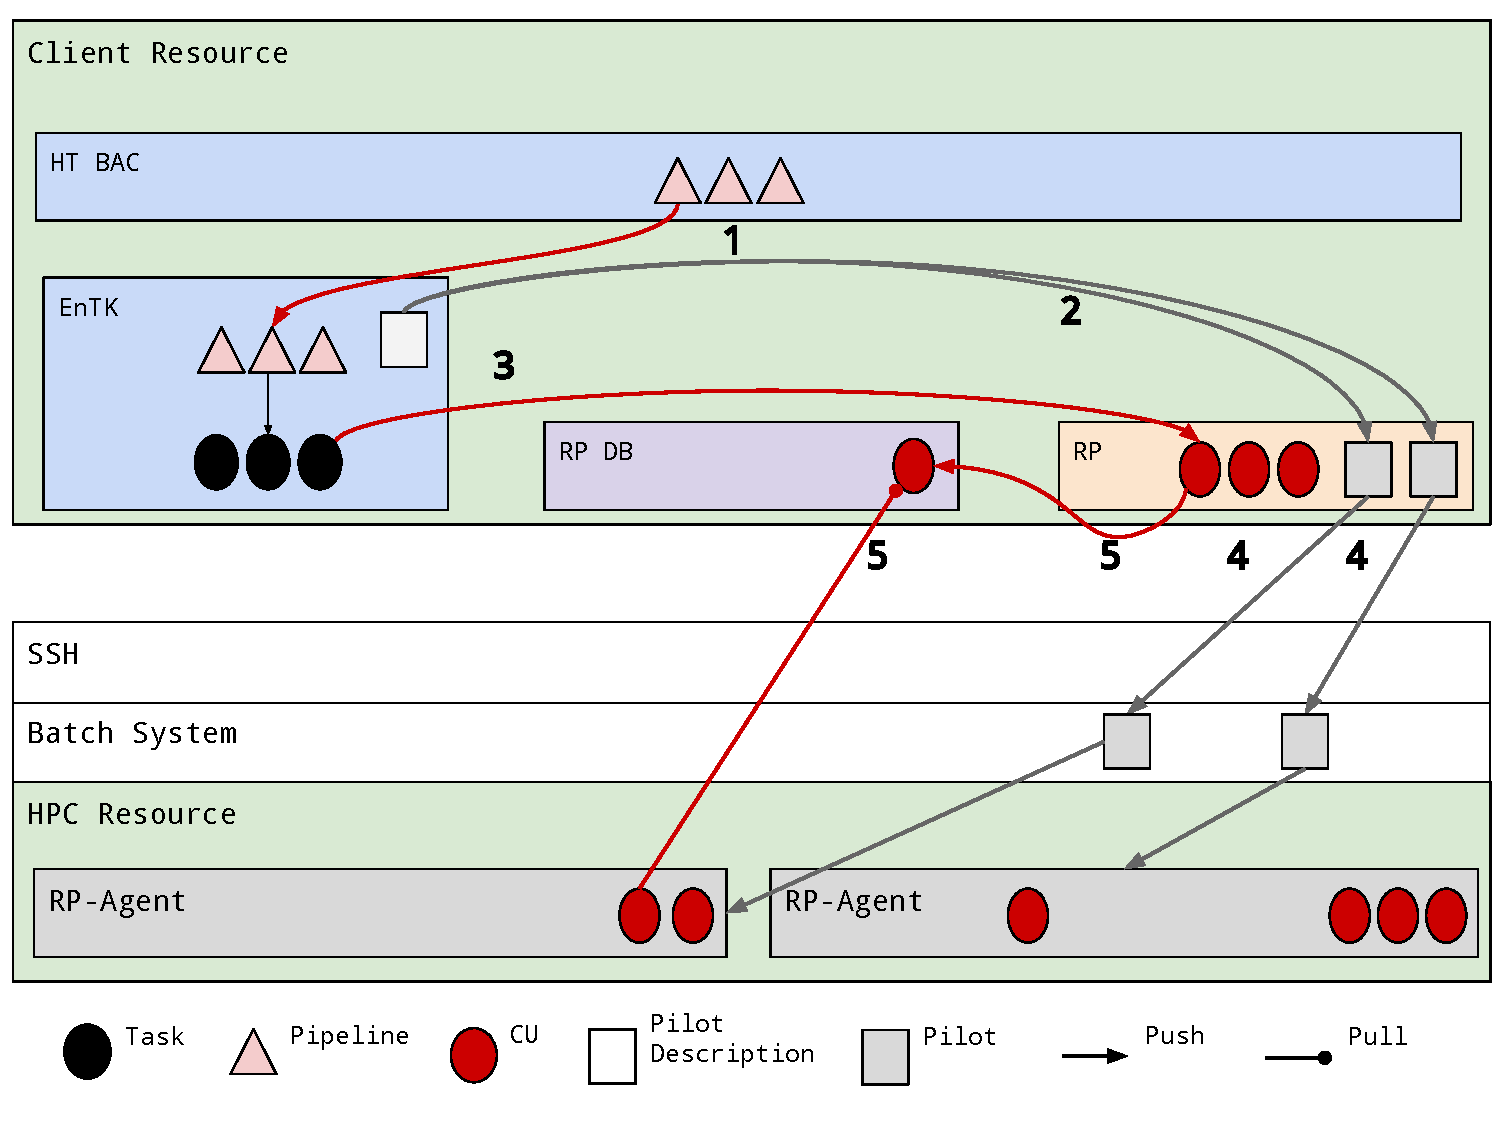
\includegraphics[width=0.5\textwidth]{FIGURES/ht-bac-rp_integration.pdf}
  \caption{Integration between HTBAC workflow and EnTK\@. Numbers indicate
  the temporal sequence of execution. The database (DB) of RADICAL-Pilot (RP)
  can be deployed on any host reachable from the resources. RP pushes compute
  units (CU) to DB and RP-Agent pulls them for execution. \dwwnote{I think CU
  needs to be defined here}\mtnote{Better?}}
  \label{figure:ht-bac_rp}
\end{figure}

% RADICAL-Cybertools provides advanced resource management capabilities and,
% thereby delivers the necessary high-throughput capabilities
% required\mtnote{Required by?}. HTBAC is integrated with the EnTK component of
% RCT\@.\mtnote{I am not sure what we want to say with this short paragraph.
% Maybe we want to expand on it or comment it out?}

% \begin{figure}[ht]
% \centering
%  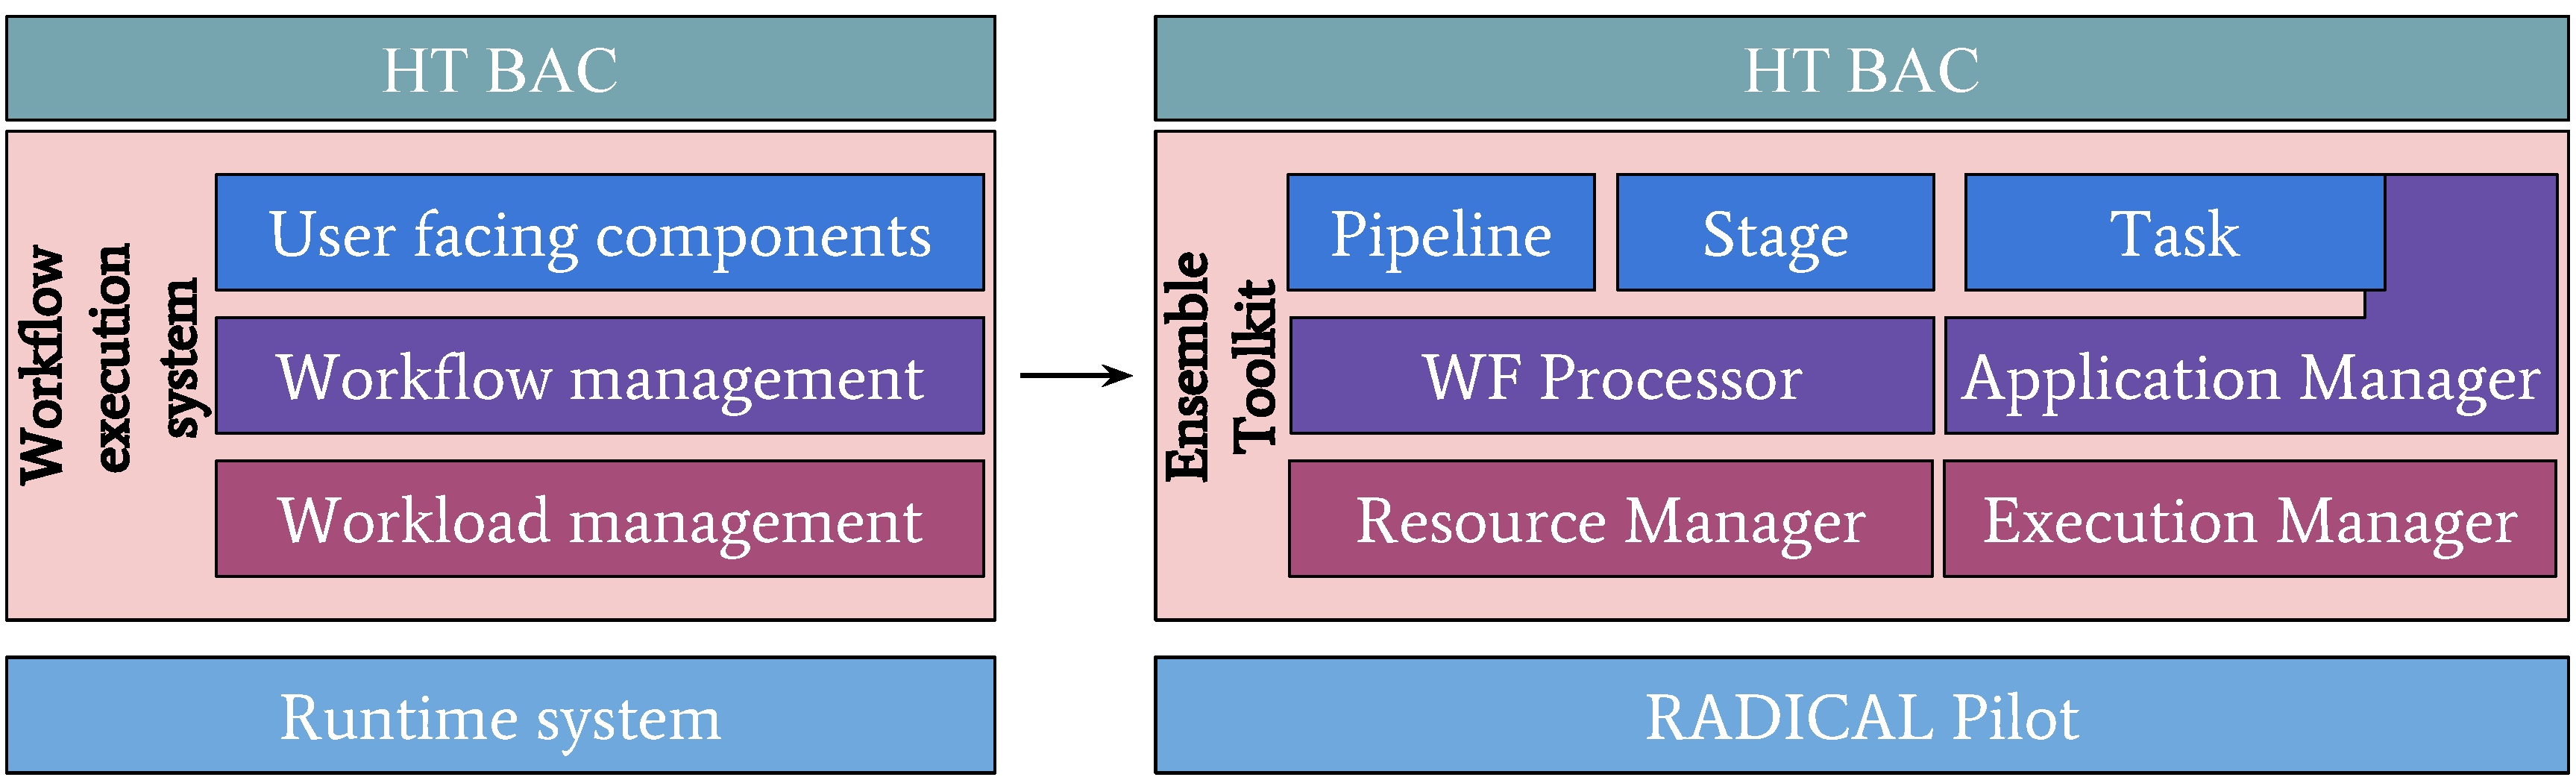
\includegraphics[width=0.5\textwidth]{FIGURES/entk_htbac_integration.pdf}
%   \caption{\bf Integration between HT-BAC workflow system and EnTK that
%   shows resource/application managers.}
%   \label{figure:ht-bac_entk}
% \end{figure}
